% !TEX root = ../thesis-sample.tex

\chapter{STANDARD MODEL} \label{chap:intro}



\section{Basic concepts}

 %%%% Teoria    2 semanas  %%%%%%%%%%%%%
 
 %%%%%%%  En paralelo
%%%%%%%%  a) Finalizar implemntacion de script para generacion de muestras en ACARUS, subir al github archivo python  
%%         b) Producir los grafficos de parametrizacion de eficiencia y resolucion de mmuones que delphes usa   delphes_card_CMS.tcl 
%%        
There are four fundamental forces at work in the universe: the strong force, the weak force, the electromagnetic force, and the gravitational force. The Standard Model includes the electromagnetic, strong and weak forces and all their carrier particles, and explains well how these forces act on all of the matter particles.

\subsection{Fundamental forces}

The fundamental forces (or fundamental interactions) of physics are the ways that individual particles interact with each other. It turns out that every single interaction observed taking place in the universe can be broken down and described by only four (well, generally four—more on that later) types of interactions:

\begin{itemize}
    \item \textbf{\textcolor{azul50}{Gravity: }} has the farthest reach, but it's the weakest in actual magnitude. It is a purely attractive force which reaches through even the "empty" void of space to draw two masses toward each other. Is described under the theory of general relativity, which defines it as the curvature of spacetime around an object of mass. This curvature, in turn, creates a situation where the path of least energy is toward the other object of mass.
    \item \textbf{\textcolor{azul50}{Electromagnetism :}} is the interaction of particles with an electrical charge. Charged particles at rest interact through electrostatic forces, while in motion they interact through both electrical and magnetic forces, is the most prevalent force in our world, as it can affect things at a reasonable distance and with a fair amount of force.
    \item \textbf{\textcolor{azul50}{Weak Interaction (or Weak Nuclear Force) :}} is a very powerful force that acts on the scale of the atomic nucleus. It causes phenomena such as beta decay. It has been consolidated with electromagnetism as a single interaction called the "electroweak interaction.", is mediated by the W boson (there are two types, the W+ and W- bosons) and also the Z boson.
    \item \textbf{\textcolor{azul50}{Strong Interaction (or Strong Nuclear Force) :}} the strongest of the forces is, keeps the nucleons (protons and neutrons) bound together. In the helium atom, for example, it is strong enough to bind two protons together even though their positive electrical charges cause them to repulse each other, the strong interaction allows particles called gluons to bind together quarks to create the nucleons in the first place. Gluons can also interact with other gluons, which gives the strong interaction a theoretically infinite distance, although it's major manifestations are all at the subatomic level.
\end{itemize}


\subsection{Particle Families}

Fundamental particles are either the building blocks of matter, called fermions, or the mediators of interactions, called bosons. Every elementary particle has associated with it a spin quantum number $s$ (often called the spin number or just the spin), where $s$ is any whole number multiple of a half. Fermions have half integral spin quantum numbers ($1/2$, $3/2$, $5/2$, etc.) and bosons have integral spin quantum numbers ($0$, $1$, $2$, etc.). No spin numbers are possible in between these. 

\begin{figure}
    \centering
    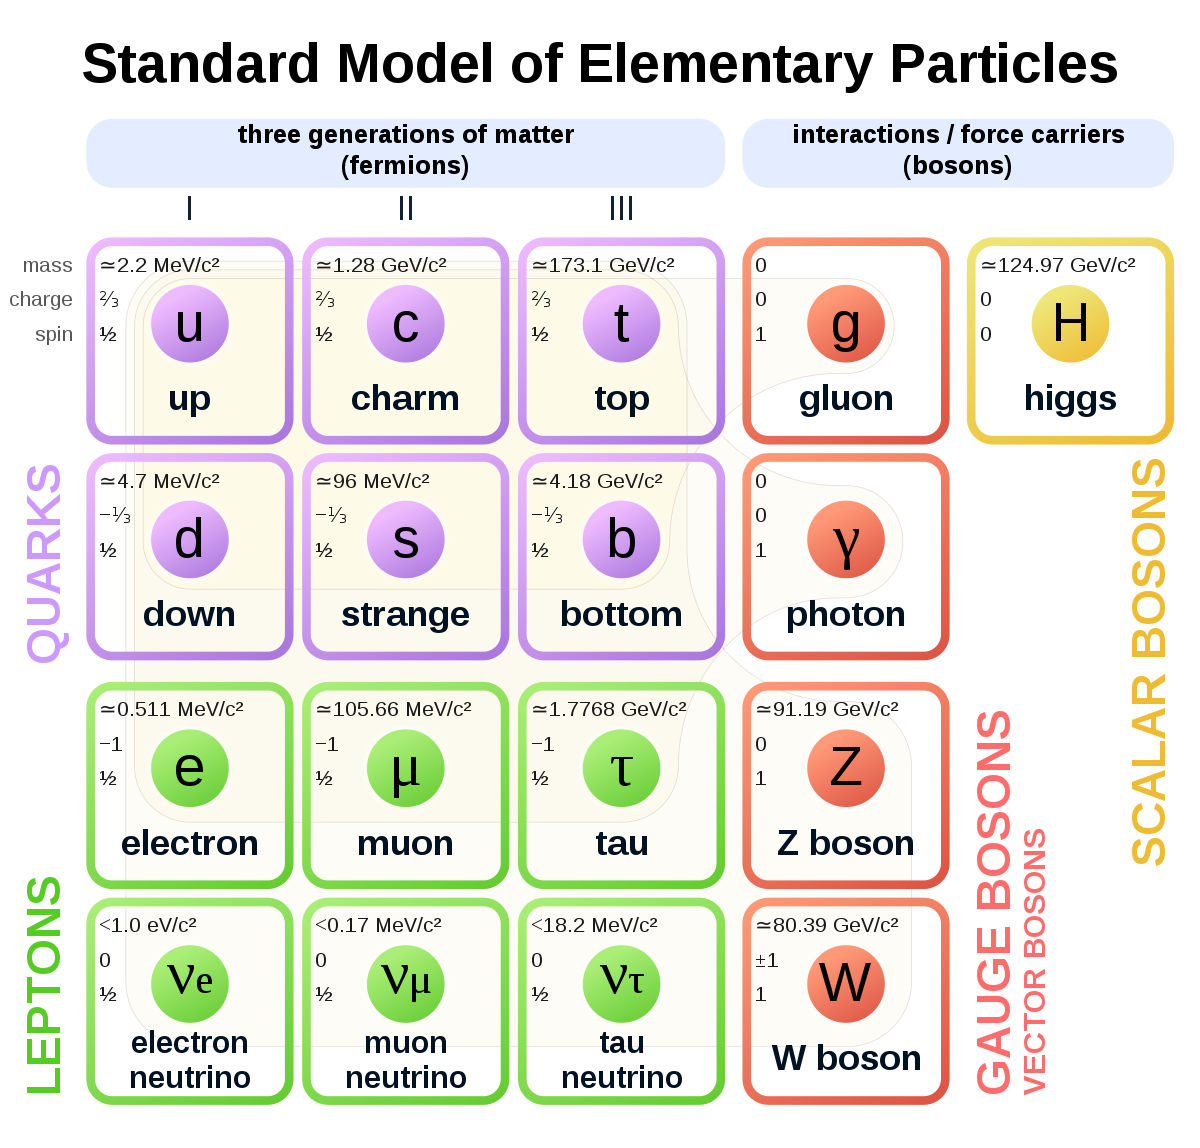
\includegraphics[width=0.7\textwidth]{tex/Chapters/Standard_Model/Imagen/Model.png}
    \caption{Standard model particles.}
    \label{fig:estandard_model}
\end{figure}

Fermions obey a statistical rule described by Enrico Fermi (1901–1954) of Italy, Paul Dirac (1902–1984) of England, and Wolfgang Pauli (1900–1958) of Austria called the exclusion principle. Simply stated, fermions cannot occupy the same place at the same time. (More formally, no two fermions may be described by the same quantum numbers.) Leptons and quarks are fermions, but so are things made from them like protons, neutrons, atoms, molecules, people, and walls. This agrees with our macroscopic observations of matter in everyday life. People cannot walk through walls unless the wall gets out of the way.

Bosons, in contrast, are have no problem occupying the same place at the same time. (More formally, two or more bosons may be described by the same quantum numbers.) The statistical rules that bosons obey were first described by Satyendra Bose (1894–1974) of India and Albert Einstein (1879–1955) of Germany. Gluons, photons, and the W, Z and Higgs are all bosons. As the particles that make up light and other forms of electromagnetic radiation, photons are the bosons we have the most direct experience with. In our everyday experience, we never see beams of light crash into one another. Photons are like phantoms. They pass through one another with no effect.

%All fundamental and composite particles have a spin quantum number s (lowercase). This is associated with a spin angular momentum S (uppercase). The SI unit of angular momentum is the kilogram meter squared per second [kgm2/s] or, equivalently, the joule second [Js], which is much too large for elementary particles. Instead ℏ (h bar), also known as the reduced Planck constant (ℏ = h/2π), is used. For reasons that are beyond the scope of this book, the spin quantum number s (which is just a number) and the spin angular momentum S (which is a number with a unit) are not numerically the same. Instead, they are related by a non-obvious equation.


\begin{table}[h!]
  \begin{center}
    \caption{Standard model particles.}
    \label{tab:table1}
    \begin{tabular}{|c|c|c|c|c|c|c|c||} 
        \hline\hline
        \multicolumn{3}{|c|}{\textbf{Family}} & \textbf{Particle} & \textbf{Spin Number} & \textbf{Charge (e)} & \textbf{Color} & \textbf{Mass}\\
        \hline
        F & Q & $u$ & Up Quarks & $1/2$ & $+2/3$ & $r, g, b$	& $2.16$ \\
        \hline
        E & U & $d$ & Down Quark & $1/2$ & $-1/3$ & $r, g, b$ & $4.67$ \\ 
        \hline
        R & A & $c$ & Charm Quark & $1/2$ & $+2/3$ & $r, g, b$ & $1,27$ \\
        \hline
        M & R & $s$ & Strange Quark & $1/2$ & $-1/3$ & $r, g, b$ & $93$ \\
        \hline
        I & K & $t$ & Top Quark & $1/2$ & $+2/3$ & $r, g, b$ & $172.9$ \\
        \hline
        O &  & $b$ & Bottom Quark & $1/2$ & $-1/3$ & $r, g, b$ & $4.18$ \\
        \hline
        N & L & $e$ & Electron & $1/2$ & $-1$ & none & $\approx 0.51$ \\
        \hline
        S & E & $\mu$ & Muon & $1/2$ & $-1$ & none & $\approx 105.65$ \\
        \hline
          & P &  $\tau$ & Tau & $1/2$ & $-1$ & none & $1776.86$ \\
        \hline
          & T & $v_e$ & Electron Neutrino & $1/2$ & $0$ & none & $<2\times10^{-6}$ \\
        \hline
          & O & $v_\mu$ & Muon Neutrino  & $1/2$ & $0$ & none & $<0.19$ \\
        \hline
          & N & $v_\tau$ & Tau Neutrino & $1/2$ & $0$ & none & $<1.2$ \\
        \hline
          & $-$ & $p$ & Proton & $1/2$ & $+1$ & none & $\approx 938.27$ \\
        \hline
          & $- $& $n$ & Neutron & $1/2$ & $0$ & none & $\approx 939.56$ \\
        \hline
        B & & $g$ & Gluon & $1$ & $0$ & 8 colors & $0$ \\
        \hline
        O & & $\gamma$ & Photon & $1$ & $0$ & none & $0$ \\
        \hline
        S & & $W$ & W Boson & $1$ & $0$ & none & $0$ \\
        \hline
        O & & $Z$ & Z Boson & $1$ & $0$ & none & $0$ \\
        \hline
        N & & $H$ & Higgs Boson & $0$ & $0$ & none & $125.1$ \\
        \hline
        \end{tabular}
  \end{center}
\end{table}

Elementary particles have an intrinsic spin angular momentum $S$. The adjective intrinsic means innate or essential to the thing itself. Elementary particles don't have spin because someone is spinning them. They just spin — or rather, they just have a measurable quantity with the same units as angular momentum. In current physics, elementary particles are featureless — like a mathematical point. In order for something to be perceived as spinning, the thing spinning would need something like a "front" and a "back". Featureless, point particles don't have anything like that. Particle physics is best described with mathematics. Spin is a convenient label for a measurable quality and not a description of reality.


\section{Description of standard model}

The standard model is the name given in the 1970s to a theory of fundamental particles and how thea
\subsection{The elements of the Lagrangian}

The Standard Model of particle physics is a quantum field theory. Therefore, its fundamental elements are quantum fields and the excitations of these fields are identified as particles. For example, the quantised excitation of the electron field is interpreted as an electron. From our viewpoint, it is not only permissible, but even advisable to speak directly of elementary particles instead of field excitations when discussing basic principles of particle physics qualitatively in high school.

The Lagrangian of the standard model is an extremely compact notation. Theoretical particle physicists normally know when to sum over which indices, what different abbreviations and derivatives mean, and when to consider each of the fundamental interactions:
\begin{equation}
    \mathcal{L} = - \dfrac{1}{4}F_{\mu v}F^{\mu v} + i\vec{\psi}{\not D} \psi + \psi_i  Y_{ij} \psi_j \phi + |D_m \phi|^2 - V(\phi)
\end{equation}
n the physics classroom, however, it is very difficult to achieve a deep-level understanding because the required mathematics skills go far beyond high-school level.

$\mathcal{L}$  stands for the Lagrangian density, which is the density of the Lagrangian function L in a differential volume element. In other words, $\mathcal{L}$  is defined such that the Lagrangian L is the integral over space of the density: $L={\int}^{}{{\text{d}}^{3}}x~\mathcal{L}$ . 
In 1788, Joseph–Louis Lagrange introduced Lagrangian mechanics as a reformulation of classical mechanics. It allows the description of the dynamics of a given classical system using only one (scalar) function L=T-V where T is the kinetic energy and V the potential energy of the system. The Lagrangian is used together with the principle of least action to obtain the equations of motion of that system in a very elegant way.

When handling quantum fields, instead of the discrete particles of classical mechanics, the Lagrangian density describes the kinematics and dynamics of the quantum system. Indeed, the Lagrangian density of quantum field theory can be compared to the Lagrangian function of classical mechanics. Hence, it is common to refer to $\mathcal{L}$  simply as 'the Lagrangian'.

The term $-\dfrac{1}{4}F_{\mu v}F^{\mu v}$ is the scalar product of the field strength tensor ${{F}_{\mu \nu}}$  containing the mathematical encoding of all interaction particles except the Higgs boson, where $\mu$ and $v$ are Lorentz indices representing the spacetime components. It contains the necessary formulation for these particles to even exist, and describes how they interact with each other. The contents differ depending on the properties of the interaction particles. For example, photons, the interaction particles of the electromagnetic interaction, cannot interact with each other, because they have no electric charge. Therefore, the contribution of the electromagnetic interaction consists only of a kinetic term, the basis for the existence of free photons. The description of gluons and the weak bosons also includes interaction terms in addition to the kinetic terms. Gluons, for example, are colour-charged themselves and can therefore also interact with each other. This leads to an exciting consequence: the Standard Model of particle physics predicts the existence of bound states consisting only of gluons, so-called 'glueballs'. However, no experiment has detected glueballs thus far.


The term $i\vec{\psi}{\not D} \psi$ describes how interaction particles interact with matter particles. The fields $\psi$ and $\bar{\psi}$  describe (anti)quarks and (anti)leptons. The bar over $\bar{\psi}$  means that the corresponding vector must be transposed and complex-conjugated; a technical trick to ensure that the Lagrangian density remains scalar and real. ${\not D}$  is the so-called covariant derivative, featuring all the interaction particles (except the Higgs), but this time without self-interactions.

The beauty of this term is that it contains the description of the electromagnetic, weak, and strong interactions. Indeed, while all three fundamental interactions are different, the basic vertices by which they can be visualised look quite similar. We will start by discussing the most important interaction of our daily lives, the electromagnetic interaction. Here, pair production or annihilation of electrons and positrons, and the absorption or emission of photons by electrons, are prominent examples. All four of these processes can be represented using Feynman diagrams with the same basic vertex.

This term $\psi_i  Y_{ij} \psi_j \phi$ describes how matter particles couple to the Brout–Englert–Higgs field phgr and thereby obtain mass. The entries of the Yukawa matrix yij represent the coupling parameters to the Brout–Englert–Higgs field, and hence are directly related to the mass of the particle in question. These parameters are not predicted by theory, but have been determined experimentally.

Parts of this term still cause physicists headaches: it is still not clear why neutrinos are so much lighter than other elementary particles, in other words, why they couple only very weakly to the BEH field. In addition, it is still not possible to derive the entries of the Yukawa matrix in a theoretically predictive way.

It is known that particles with high mass, in other words with a strong coupling to the Brout–Englert–Higgs field,also couple strongly to the Higgs boson. This is currently being verified experimentally at the LHC, where Higgs bosons are produced in particle collisions. However, Higgs bosons transform into particle–antiparticle pairs after about 10-22 s. Depending on their mass, i.e. their coupling parameter,certain particle–antiparticle pairs are much more likely, and thus easier to observe experimentally, than others.nThis is because the coupling parameter, which describes the coupling to the Higgs boson, is simply the mass of the particle itself. The Higgs boson is thus more likely to be transformed into pairs of relatively more massive particles and anti-particles. Measurements by the ATLAS detector show, for example, evidence of the direct coupling of the Higgs boson to tauons.

The term $|D_m \phi|^2$ describes how the interaction particles couple to the BEH field. This applies only to the interaction particles of the weak interaction, which thereby obtain their mass. This has been proven experimentally, because couplings of W bosons to Higgs bosons have already been verified. Photons do not obtain mass by the Higgs mechanism, whereas gluons are massless because they do not couple to the Brout–Englert–Higgs field.

The term $V(\phi)$ describes the potential of the BEH field. Contrary to the other quantum fields, this potential does not have a single minimum at zero but has an infinite set of different minima. This makes the Brout–Englert–Higgs field fundamentally different and leads to spontaneous symmetry-breaking (when choosing one of the minima). As discussed for terms 4 and 6, matter particles and interaction particles couple differently to this 'background field' and thus obtain their respective masses. This also describes how Higgs bosons couple to each other. The Higgs boson, the quantised excitation of the BEH field, was experimentally confirmed at CERN in 2012. In 2013, François Englert and Peter Higgs were awarded the Nobel Prize in Physics for the development of the Higgs mechanism.













El experimento Solenoide Compacto de Muones o \CMS(\textbf{C}ompact \textbf{M}uon \textbf{S}olenoid) tiene la capacidad de cubrir un amplio rango de procesos físicos, este experimento consiste de varios subsistemas los cuales están diseñados para la identificación de prácticamente todas las partículas del modelo estándar. Para su diseño se tomó en cuenta cómo cada partícula interacciona con la materia, por ejemplo las partículas cargadas son identificadas por medio de detectores a base de silicio y de gas noble, permitiendo determinar con precisión el tiempo y localización de las partículas. La variedad de interacciones por tipo de partícula se puede ver en la Fig. \ref{cms}.

\begin{figure}[!ht]
\centering
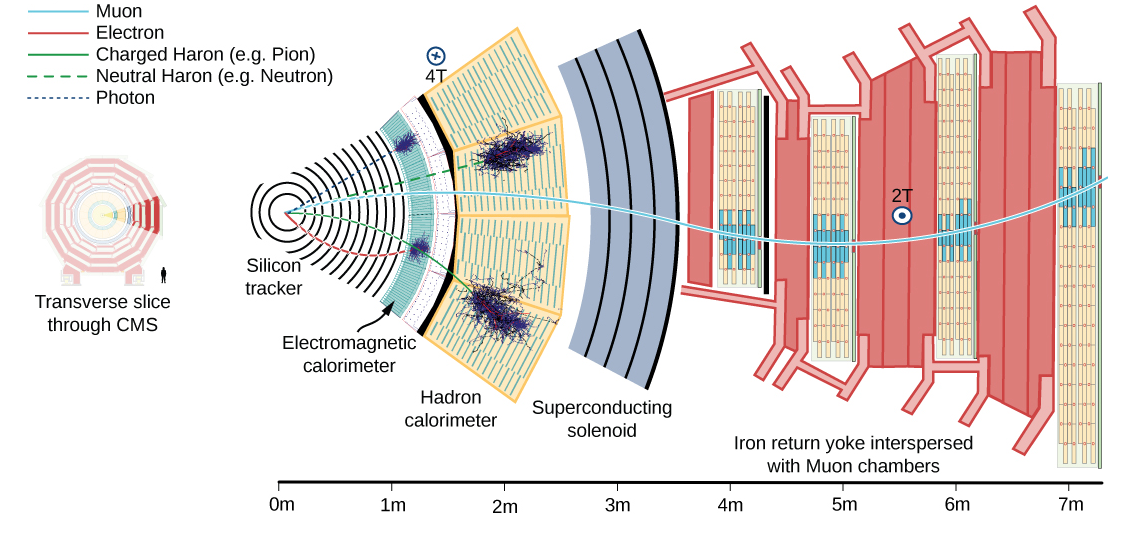
\includegraphics[width=1\textwidth]{Cap2/imagenes/CMS_interaction.png}
\caption[Detector de solenoide de muón compacto. El detector consta de varias capas, cada una responsable de medir diferentes tipos de partículas.]{Detector de solenoide de muón compacto. El detector consta de varias capas, cada una responsable de medir diferentes tipos de partículas.\footnotemark}
\label{cms}
\end{figure}

\footnotetext{Página de origen: \href{http://ippog.web.cern.ch/resources/2011/cms-slice-july-2010-version}{http://ippog.\-web.\-cern.\-ch/\-resources/\-2011/\-cms-\-slice-\-july-\-2010-\-version}}

El \CMS ~ es un detector de propósito general, capaz de estudiar múltiples aspectos de las colisiones de protones hasta 14 TeV, este contiene sistemas para medir la energía y la cantidad de movimiento de fotones, electrones, muones y otras partículas producto de las colisiones \citep{cms_1}. La capa detectoras (ver Fig. \ref{cms}) se pueden dividir en: 
\begin{itemize}
\item  \textbf{El detector de trazas de Silicio (The Silicon tracker):} para calcular el momento de una partícula es rastrear su camino a través de un campo magnético; ~ cuanto más curvaba el camino, menos impulso tenía la partícula. El detector de trazas \CMS ~ registra los caminos tomados por las partículas cargadas al encontrar sus posiciones en varios puntos clave. De esta forma se reconstruyen los caminos de muones de alta energía, electrones y hadrones (partículas formadas por quarks), así como ver las huellas que provienen de la descomposición de partículas de vida muy corta.

El detector de trazas \CMS ~ está hecho completamente de silicio: los píxeles, en el núcleo mismo del detector y que se ocupan de la mayor intensidad de partículas, y los detectores de microstrip de silicio que lo rodean. A medida que las partículas viajan a través del detector, los píxeles y las microstrips producen pequeñas señales eléctricas que se amplifican y detectan. %El rastreador emplea sensores que cubren un área del tamaño de una cancha de tenis, con 75 millones de canales de lectura electrónica separados: en el detector de píxeles hay unas 6,000 conexiones por centímetro cuadrado.

%\textbf{Actualización de Alta Luminosidad: }

%La actualización esperada de \textbf{HL-}\LHC~ aumentará el número de interacciones hasta el punto en que la ocupación excesiva reduciría significativamente la efectividad de la búsqueda de pistas. Se planea una actualización para aumentar el rendimiento y la tolerancia a la radiación del rastreador.

\item \textbf{Calorímetro electromagnético} o \textbf{ECAL} (\textbf{E}lectromagnetic \textbf{CAL}orimeter): componente diseñado para medir con alta precisión las energías de electrones y fotones, está construido a partir de cristales de plomo tungstato $\mathbf{PbWO_4}$, por ser un material extremadamente denso pero ópticamente transparente, de aquí que se utilize para detener partículas de alta energía, este material está hecho principalmente de metal y es más pesado que el acero inoxidable. Para mayor precisión espacial, el \textbf{ECAL} también contiene detectores de ``preshower'' que se encuentran frente a las tapas finales, permitiendo distinguir entre fotones individuales de alta energía (a menudo signos de física emocionante) y los pares cercanos menos interesantes de fotones de baja energía. Está calibrado para discriminar entre de piones y fotones.

\item \textbf{El calorímetro de hadrones} o \textbf{HCAL}(\textbf{H}adronic \textbf{CAL}orimeter): mide la energía de los hadrones, además, proporciona una medición indirecta de la presencia de partículas no cargadas que no interactúan, como los neutrinos. Consta de capas de material denso (latón o acero) intercaladas con baldosas de centelleadores de plástico, leídas a través de fibras que cambian la longitud de onda mediante fotodiodos híbridos, de esta forma se permite la máxima cantidad de material absorbente dentro de la bobina magnética.

\item \textbf{Solenoide supercondutor (Superconducting Solenoid):} es el dispositivo central alrededor del cual se construye el experimento, con un campo magnético que %de 4 Tesla 
permite determinar la relación carga/masa de partículas a partir de la pista curva que siguen en el campo magnético. Tiene $13~m$ de largo y $6~m$ de diámetro, y sus bobinas de niobio-titanio superconductoras refrigeradas estaban destinadas originalmente a producir un campo magnético %de hasta $4~T$
. Es componente tiene la función de doblar los caminos de las partículas que emergen de colisiones, permitiendo determinar con la trayectoria curvada por el campo magnético el impulso, combinado con mediciones de posición de alta precisión en los detectores de muones, esto permite una alta medición en sus resultados.

\item \textbf{Los detectores de muones :} dedicado a la detección de muones, siendo estas partículas cargadas y 200 veces más masivas que los electrones y positrones, se espera que se produzcan en la descomposición de una serie de posibles partículas nuevas. Debido a que los muones pueden penetrar varios metros de hierro sin interactuar, ninguno de los calorímetros de \CMS ~los detiene. Por lo tanto, las cámaras para detectar muones se colocan en el borde mismo del experimento, donde son las únicas partículas que pueden registrar una señal. Para identificar muones y medir sus momentos, \CMS ~ utiliza tres tipos de detectores: 
\begin{itemize}
\item \textbf{Tubos de deriva} o \textbf{DT}(\textbf{D}rift \textbf{T}ubes) : se usan para mediciones de trayectoria precisas en la región central del barril.
\item \textbf{Cámaras de banda catódica} o \textbf{CSC}(\textbf{C}athode \textbf{S}trip \textbf{C}hambers) : se usan para mediciones de trayectoria precisas en los extremos del barril. 
\item \textbf{Cámaras de placas resistivas} o \textbf{RPC}(\textbf{R}esistive \textbf{P}late \textbf{C}hambers) : proporcionan una señal rápida cuando un muón pasa a través del detector.
\end{itemize}

\end{itemize}




%\begin{figure}[ht]
%\centering
%\includegraphics[width=1\textwidth]{Analisis_y_Resultados/imagenes/Momentum_resolution_of_Muon.png}
%\caption{Comparación. Generados con python 2.7.}
%%\label{Compara_sol_muon}
%\end{figure}
%
%\begin{figure}[ht]
%\centering
%\includegraphics[width=1\textwidth]{Analisis_y_Resultados/imagenes/Tracking_of_Muon.png}
%\caption{Comparación. Generados con python 2.7.}
%%\label{Compara_track_muon}
%\end{figure}
%
%\begin{figure}[ht]
%\centering
%\includegraphics[width=1\textwidth]{Analisis_y_Resultados/imagenes/Eficiencia_of_Muon.png}
%\caption{Comparación. Generados con python 2.7.}
%%\label{Compara_track_muon}
%\end{figure}

\subsection{Actualizando \CMS}


\begin{figure}[!h]
\centering
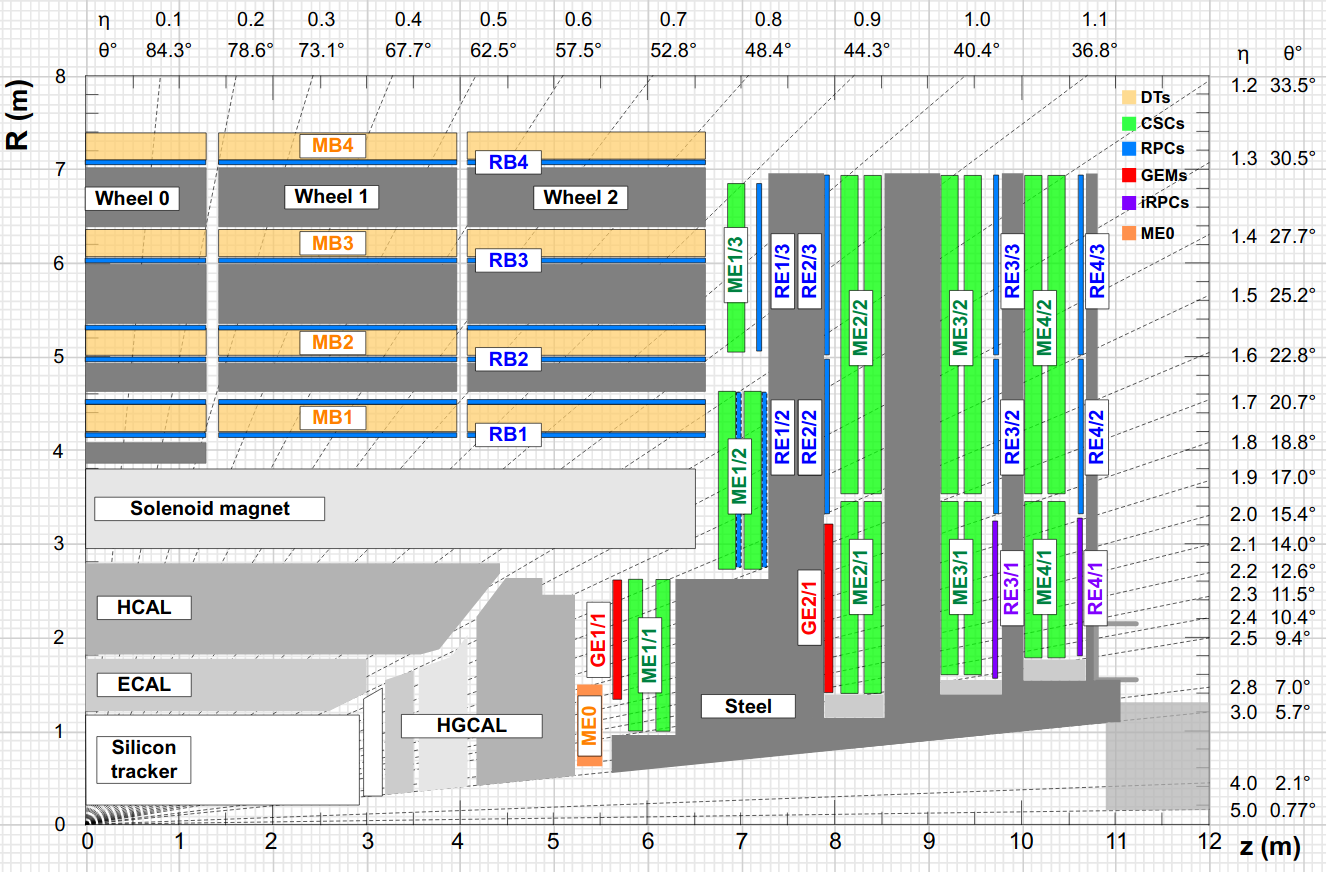
\includegraphics[width=.95\textwidth]{Cap2/imagenes/camaraZ.png}
\caption[Una sección transversal R-z de un cuadrante del detector \CMS.]{Una sección transversal R-z de un cuadrante del detector \CMS.\footnotemark.}
\label{transversal}
\end{figure}
\footnotetext{Sacada de la referencia \cite{hlhlc}}
El detector de trazas de silicio %en Run-2 
es reemplazado antes del inicio de la Fase 2, ya que se esperan daños por radiación significativos al final de Run-3. Para mantener óptima la reconstrucción se disminuye el tamaño de píxel y se acorta el tiempo de respuesta. Además, será posible una medición de momento en unos pocos microsegundos, permitiendo mejoras en la resolución $P_T$. %, y esta información se puede usar en el Level-1 (L1) ``trigger''. Las mejoras en la resolución $P_T$ resultando en las actualizaciones  combinadas del rastreador y los sistemas de muones, el umbral de $P_T$ se mantiene bajo a pesar de la alta tasa en \textbf{HL-}\LHC.

En la actualización realizada durante la Fase 1 resultó en la incorporación de nuevas cámaras \textbf{RPC} mejoradas se denominan \textbf{iRPC} (ver Fig. \ref{transversal}), que se instalarán junto a las cámaras \textbf{CSC} (\textbf{C}athode \textbf{S}trip \textbf{C}hamber) \textbf{ME3/1} y \textbf{ME4/1}. Las marcas \textbf{RPC} en la Fig. \ref{transversal} se refiere a las cámaras \textbf{RPC} ya presentes en el año 2017. Los nuevos detectores de muones que se instalarán como parte de las actualizaciones del detector (\textbf{GEM} y \textbf{iRPC}) están diseñados para mantener un rendimiento excelente durante toda la operación del\textbf{ HL-}\LHC. Para proyectar el deterioro a largo plazo de los actuales detectores de muones y componentes electrónicos durante los próximos 20 años, se ha desarrollado un modelo de envejecimiento, basado en tasas de falla medidas y estimadas en función de la dosis y el tiempo de radiación, estos se reportan en la referencia \cite{hlhlc}. Los estudios demuestran claramente que las actualizaciones propuestas son necesarias para mantener el rendimiento actual del sistema de muones.

\begin{table}[!h]
\small
\centering
\begin{tabular}{|cccccccc|}
\toprule
%Variable &  \multicolumn{7}{c}{}\\
Detector & \textbf{DT} & \textbf{CSC} & \textbf{RPC} & \textbf{iRPC} & \textbf{GE1/1} & \textbf{GE2/1} & \textbf{ME0}\\ 
\midrule
rango de $\eta$ & 0-1.2 & 0.9-2.4 & 0-1.9 & 1.8-2.4 & 1.6-2.15 & 1.6-2.4 & 2.0-2.8\\ 
\bottomrule
\end{tabular}
\caption{Rango de detección de la pseudorapidez para los componentes del detector \CMS.}
\label{camara}
\end{table}


El objetivo del programa \LHC ~ de Alta Luminosidad o \textbf{HL}(\textbf{H}igh \textbf{L}uminosity) es recopilar una luminosidad integrada de $3000 ~ fb^{-1}$, opcionalmente hasta $4500 ~ fb^{-1}$, en aproximadamente ocho años de operaciones a partir de 2028 y con una luminosidad máxima de $7.5 \times 1034~cm^{-2}s^{-1}$. El aumento de la luminosidad instantánea dará como resultado hasta $200$ colisiones inelásticas protón-protón por cruce de racimo (pileup) mientras que la luminosidad integrada conducirá a un entorno de radiación hostil sin precedentes. %En el punto más expuesto en el volumen del Rastreador, a $r \simeq 3 ~ cm$ de la línea de luz, la fluencia esperada después de 3000 fb − 1 alcanzará 2.3 × 10161 MeV neq / cm2 y la dosis ionizante total correspondiente (TID) 12 MGy.

El diseño esperado después de Fase 2 del detector de trazas se muestra en la Fig. \ref{track}, la región interna o \textbf{I}nner \textbf{T}racker (\textbf{IT}), donde $r < 20 ~ cm$($r < 30 ~ cm$ para $|z|> 120 ~ cm$), se espera una instrumentaria con alta granularidad detectores de píxeles que garantizan un reconocimiento de patrones eficiente en el entorno de alta densidad de pistas para la de \textbf{HL}. %La región del Rastreador externo o \textbf{OT}(\textbf{O}uter \textbf{T}racker) se instrumentará con módulos pt que proporcionan una reducción de datos en el detector aO (10) para que las mediciones precisas de las trayectorias de partículas cargadas del Rastreador se puedan usar en el disparador de Nivel 1 (L1) del Experimento CMS. 
Específicamente, las características principales del detector actualizado serán:
\footnotetext{Adaptada de la Fig. 1 de la referencia \cite{HL_LHC_1}}
\begin{itemize_f}
\item Contribuir a que el disparador $L1$ mida a 40 MHz el momento de partículas cargadas y rechace aquellas con $P_T < 2$ GeV.
\item Aumentar la eficiencia de detección para valores de $|\eta| < 4$ que previamente era de $|\eta| < 2.4$. 
\item Garantizar una medición precisa del momento y mantener un bajo nivel de rastreos falsos mediante una óptimización de diseño y una reducción del ``\textit{material budget}''.
\end{itemize_f}

\begin{figure}[!h]
\centering
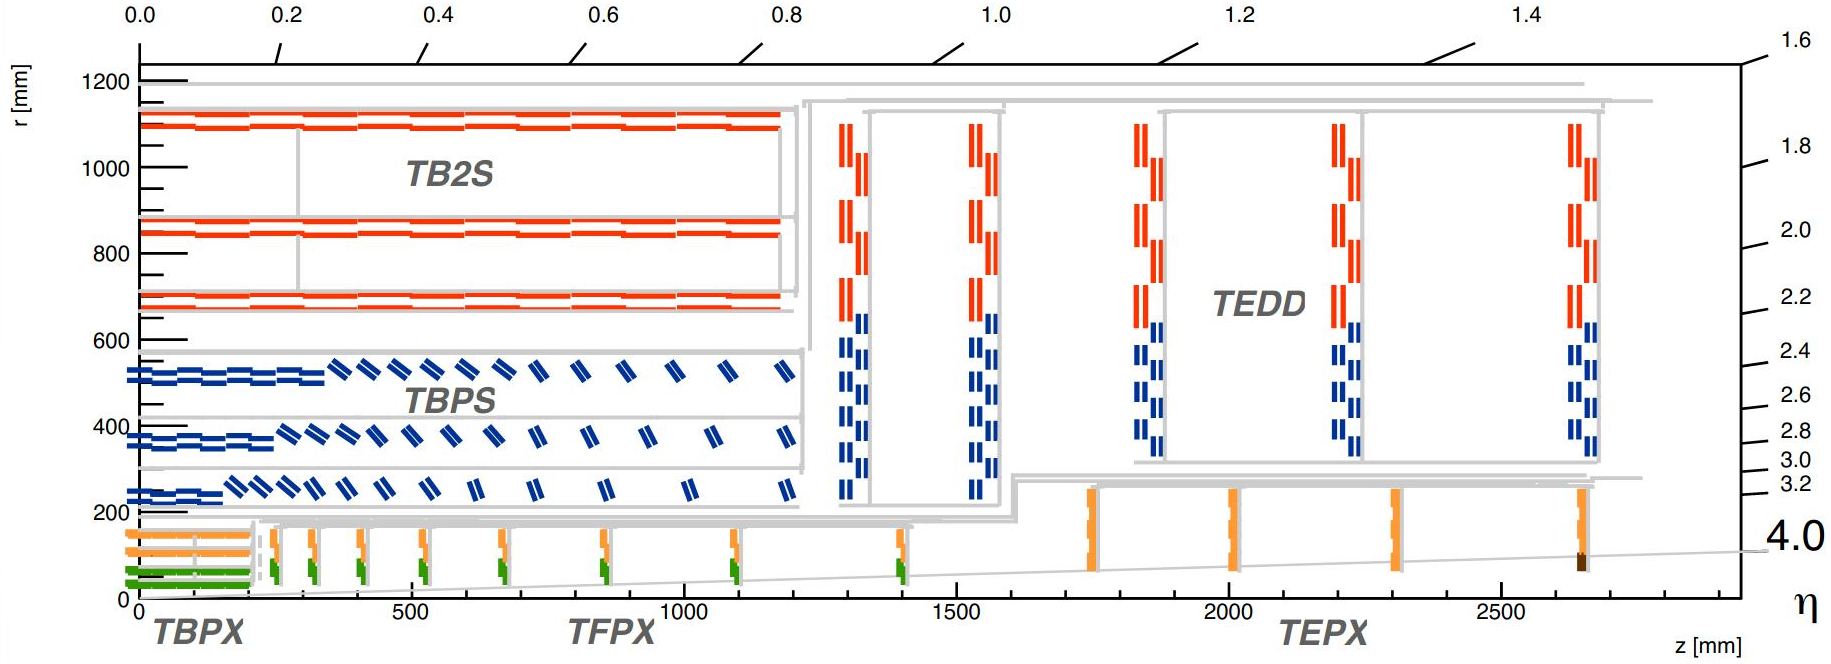
\includegraphics[width=.95\textwidth]{Cap2/imagenes/track.png}
\caption[Diagrama de una cuarta parte del diseño del detector de trazas \CMS ~ para \LHC ~ en la dirección $z$ del mismo. Los módulos de chips de lectura internos o Inner Tracker 1x2 y 2x2 se muestran en verde y amarillo respectivamente, los módulos externos o Outer Tracker PS y 2S en azul y rojo.]{Diagrama de una cuarta parte del diseño del detector de trazas \CMS ~ para HL-\LHC ~ en la dirección $z$ del detector. Los módulos de chips de lectura internos o Inner Tracker 1x2 y 2x2 se muestran en verde y amarillo respectivamente, los módulos externos o Outer Tracker PS y 2S en azul y rojo.\footnotemark.}
\label{track}
\end{figure}

\subsection{Identificación y Reconstrucción de Muones}

La identificación de partículas es parte del proceso de análisis y estudio en el \LHC, para hacer eficiente el proceso de detección, algoritmos y nuevos conceptos tuvieron que definidos e implementados para un aprovechamiento del equipamiento, con la intención de maximizar las observaciones válidas de las partículas que se estudian, en especial la identificación de procesos en los que intervienen los muones sigue siendo uno de los objetivos del proyecto por lo que se hace necesario analizar parte del proceso de identificación y reconstrucción de muones.

\subsubsection{Reconstrucción de muones.}
La reconstrucción de muones es resultado de la implementación de un algoritmo sistémico que se ejecuta en un software de reconstrucción que utiliza información de impacto para rechazar objetos físicos, muones. La reconstrucción de muones se realiza en el detector de trazas y el sistema de muones, y se compone de tres pasos secuenciales: reconstrucción local, reconstrucción independiente y reconstrucción global. 

\begin{figure}[!t]
\centering
\includegraphics[width=.90\textwidth]{Cap2/imagenes/Tracking_of_Muon.png}
\caption{Eficiencia de reconstrucción %Muon tracking efficiency
de los muones en condiciones de Run-2 (izquierda) y HL (derecha).}
\label{Compara_track_muon}
\includegraphics[width=.90\textwidth]{Cap2/imagenes/Momentum_resolution_of_Muon.png}
\caption{Resolución en la medición del momento de los muones %Momentum resolution for muons
en condiciones de Run-2 (izquierda) y HL (derecha).}
\label{Compara_sol_muon}
\end{figure}
En la Fig. \ref{Compara_track_muon} se puede observar como aumenta la capacidad del experimento \CMS ~ para diferentes condiciones del experimento, en esta se evidencia el aumento de la detección de los muones con valores de $\eta > 2.4$, esto es parte del proceso de actualización a Alta Luminosidad. Además la resolución de los valores de momento reconstruidos de los muones en las condiciones actuales del experimento y en las previstas de alta luminosidad se puede ver en la Fig. \ref{Compara_sol_muon}, es clara la disminución del error para la región común ($0<\eta < 2.4$).

La reconstrucción local utiliza la información del golpe recopilada por el sistema muon para construir pistas; entonces, la información de la pista, como entrada, se alimenta al algoritmo de reconstrucción independiente. La reconstrucción global utiliza no solo información de reconstrucción independiente, sino también golpes de seguimiento de silicio. La reconstrucción del muón coincide con el camino del muón desde el sistema de muones al detector de trazas de silicio. La reconstrucción independiente se llama reconstrucción de Level-2 y la reconstrucción global se llama reconstrucción de Level-3. Los muones reconstruidos por reconstrucción independiente y global se denominan, respectivamente, muones independientes y muones globales.



\subsubsection{Identificación de muones.}

La ``D0 muon ID'' es un algoritmo utilizado para seleccionar candidatos a muones y es un algoritmo complementario para la reconstrucción estándar. A diferencia de la reconstrucción estándar, utiliza información de energía adicional de \textbf{ECAL} y \textbf{HCAL}, y está al revés en términos de información del detector. Muon Identificación primero reconstruye las pistas de los detectores de trazas de silicio y luego utiliza la información de la \textbf{ECAL} y la \textbf{HCAL}.

También se consideran los detectores que no están asociados con ningún rastro de muones independiente, lo que le permite reconstruir algunos muones de $p_\mathbf{T}$ bajos sin suficiente energía para alcanzar el sistema muónico. Estos bajos $p_\mathbf{T}$ muones pueden no ser reconstruidos como muones globales, pero son identificados por el algoritmo de identificación de muones. Los muones reconstruidos por el algoritmo de identificación se denominan muones rastreados (``tracker muons'').

\subsubsection{Aislamiento de muones}


Ya que se espera que los muones provenientes de la señal estén aislados sin depósitos sustanciales en el detector de trazas y en los calorímetros, entonces definiéndose un cono alrededor del muón como se muestra en la Fig. \ref{torre}a y considerando las posiciones del detector de trazas y calorímetro dentro de él, se calcula la energía transversal total $E_\mathbf{T}$

El muón se considera aislado si estas deposiciones no exceden algunos umbrales. La aplicación del aislamiento en la selección de muones ayuda a reducir el fondo proveniente de muchas fuentes, especialmente \textbf{QCD}, pero también de objetos pesados como $Z$ y $W+$jets 
\begin{figure}[!t]
\centering
(a)
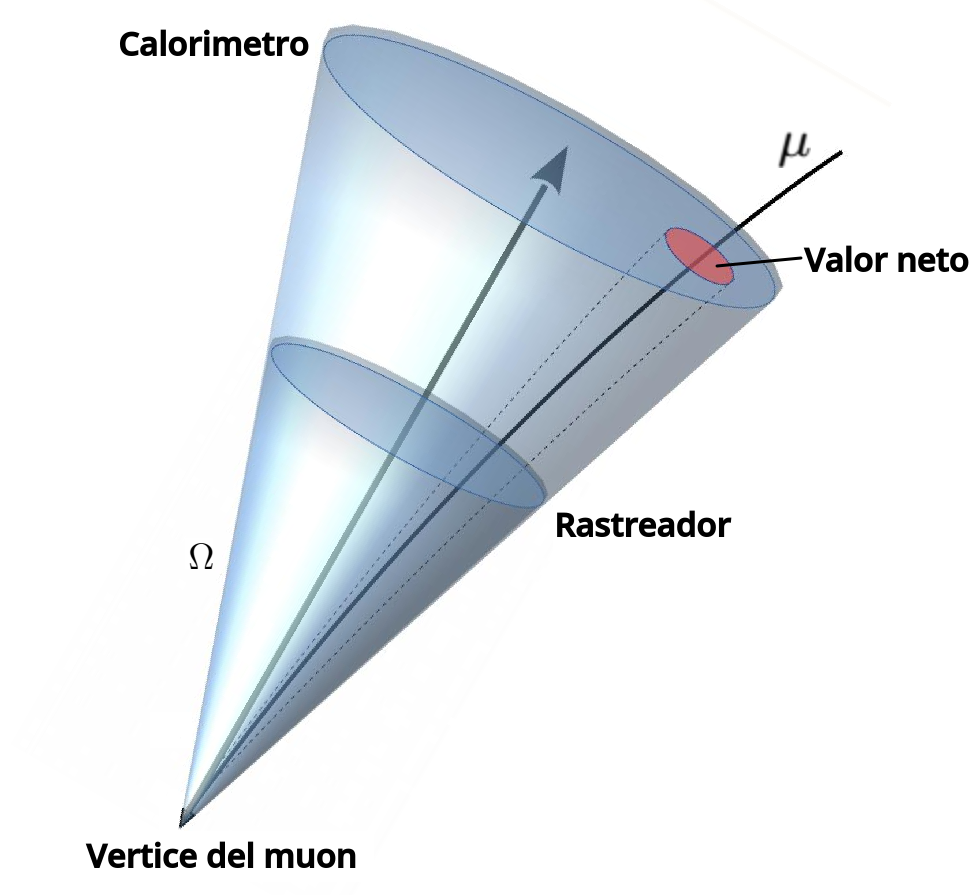
\includegraphics[width=.45\textwidth]{Cap2/imagenes/cono_mu.png}
(b)
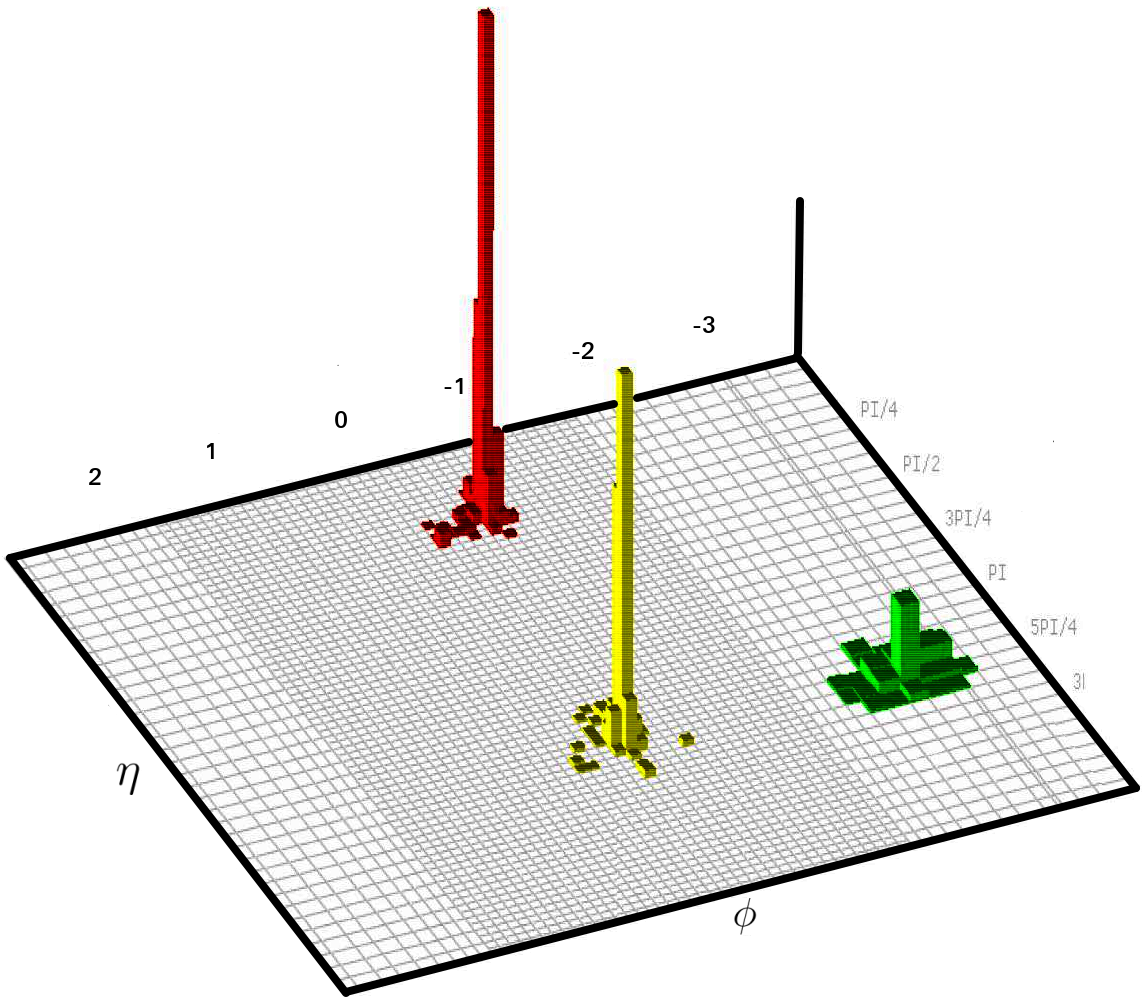
\includegraphics[width=.45\textwidth]{Cap2/imagenes/plano.png}
\caption{(a) Ilustración esquemática del cono de aislamiento. La dirección del muón en el vértice define el eje del cono; (b) Segmentación en el plano $\eta \times\phi$ en CMS sobre el que se muestran torres de energía definidas para coincidir con la segmentación o resolución del calorímetro, basada en la Fig. 1 de la referencia \cite{tower_1}.}
\label{torre}
\end{figure}
En muchas investigaciones, se han estudiado y aplicado muchos criterios de aislamiento, utilizando información de los detectores. La elección más robusta y típica realizada es aquella que contemple a todos los detectores, para tener un análisis con un criterio de aislamiento híbrido, dependiente de $p_T$, basado en una combinación de información en el detector de trazas, \textbf{HCAL} y \textbf{ECAL}. Específicamente, la variable de aislamiento basada en el detector de trazas $SumP_T$ se define como la suma escalar del $p_T$ en el plano $\eta \times \phi$ del detector de trazas dentro del cono correspondiente a $\Delta R<0.3$ donde:
\begin{equation}\label{deltaR}
\Delta R = \sqrt{\Delta \phi^2 + \Delta\eta^2}
\end{equation}
donde $\eta$ es la pseudorapidez y $\phi$ el ángulo azimutal. Entonces, alrededor del muón ($0.01 < \Delta R < 0.3$ en el plano del detector) se define como:
\begin{equation}\label{sumPT}
SumP_T =\sum_{0.01<\Delta R <0.03}^\mathbf{tracking} p_T^\mathbf{tracking}
\end{equation}
En los calorímetros, las variables $hadE_T$ y $emE_T$, correspondientes a la \textbf{HCAL} y \textbf{ECAL} respectivamente, se calculan como la suma escalar de la energía transversal depositada sobre las torres de los calorímetros (ver Fig. \ref{torre}b) en un cono de $\Delta R < 0.3$ alrededor del muón:
\begin{eqnarray}
hadE_T =\sum_{0.01<\Delta R <0.03}^\mathbf{HCAL} E_T^\mathbf{torres}  ~~~~~ y ~~~~~ emE_T =\sum_{0.01<\Delta R <0.03}^\mathbf{ECAL} E_T^\mathbf{torres} 
\end{eqnarray}
El aislamiento del detector de trazas es más importante que el de los calorimétricos, pero una combinación de los posibles aislamiento unidos a \textbf{ECAL} y \textbf{HCAL} funciona mejor. Esta combinación se construye como:
\begin{equation}\label{iso}
Iso_\mu = hadE_T + emE_T  +Sump_T
\end{equation}





\subsubsection{Eficiencia Muon}

Las secciones anteriores describen brevemente cada parte del experimento \CMS ~ desde la vía interna, más cercana a la línea del haz, hasta el sistema de muones más externo. Muchos análisis físicos requieren la probabilidad de que un muón se reconstruya como un objeto muón, dado que el muón se produce en un evento. En general, esa probabilidad se llama eficiencia, siendo la relación entre el número de muones que pasan los criterios deseados y el número total de muones producidos, se puede definir como:
\begin{equation}
\epsilon_\mu = \epsilon_\mathbf{track} \cdot \epsilon_\mathbf{id} \cdot 
\epsilon_\mathbf{iso} \cdot  \epsilon_\mathbf{trig}
\end{equation}
donde $\epsilon_\mathbf{track}$ es la eficiencia del detector de trazas de muones, es decir, la probabilidad de que un muón producido en un evento también se reconstruya%como un rastreador de silicio para detección de muones
; $\epsilon_\mathbf{id}$ es la eficiencia de identificación del muón, o sea, la probabilidad de que un muón pase por un grupo de criterios de selección, dado que es un muón reconstruido; $\epsilon_\mathbf{iso}$ es la eficiencia de aislamiento del muón, la probabilidad de que un muón reconstruido esté aislado. $\epsilon_\mathbf{trig}$ es la eficiencia del disparador, la probabilidad de que un muón reconstruido y aislado se dispare en términos de un umbral de $p_{T}$ dado.

La eficiencia de la reconstrucción muónica depende de dos factores principales: la configuración de los detectores \CMS ~ y el valor del  momento transversal $p_\mathbf{T}$ de los muones. Esta eficiencia está influenciada por la ruta a través de la cual pasa un detector, porque el detector no es homogéneo, por lo tanto, la pseudoapidez $|\eta|$ y el ángulo azimutal $\phi$ desempeñan un papel en la decisión de la eficiencia del muón. Como el detector es muy simétrico con respecto a $\phi$ no influye significativamente en la eficiencia del muón. La $p_T$ de los muones decide si tienen suficiente energía para llegar al sistema muónico, debido a que los muones independientes necesitan más de una estación para ser alcanzados en el sistema muónico, los muones con bajo $p_T$ no pueden reconstruirse como muones independientes. Toda esta información es resumida en archivos $\mathbf{*.tcl}$ característicos para uso del programa \textbf{Delphes}, aunque solo de forma básica ya que este describe de forma simplista y general el sistema.

\begin{figure}[!t]
\centering
\includegraphics[width=1\textwidth]{Cap2/imagenes/Eficiencia_of_Muon.png}
\caption{Eficiencia de reconstrucción de los muones %Muon efficiency
en condiciones de Run-2 (izquierda) y HL (derecha).}
\label{Compara_eficiencia_muon}
\end{figure}


%Como se puede observar en la Fig. \ref{Compara_eficiencia_muon} se extiende como es esperado la eficiencia para valores de $\eta > 2.4$ en la configuración de Alta Luminosidad, esto como resultado de la actualización pĺanificada por el proyecto.











 
\chapter{Beyond Standard Model} 

\section{Dark matter}

Dark matter has become such an established paradigm in modern astroand particle physics that its existence is generally accepted with little explanation. Such blithe and widespread adoption of a cosmology in which an unknown matter plays the pivotal role has led some to become a little sceptical about its existence. It is worth reminding ourselves, from time to time, of the strong and compelling evidence on which this paradigm actually stands. As it so happens, we will also pick up a good deal of information along the way about what properties dark matter must have.

\section{Dark-SUSY model}

\section{Previous searches}

%%%%%%%%%%%%%%%%%%%%%%%%%%%%%%%%%%%%%%%%%%%


\chapter{Delphes Simulation}

\section{Muon efficiency parametrization}

\section{Integration of Dark-SUSY model}


\chapter{CMS detector}

\subsection{Muon system}

\chapter{High Luminosity Era}




